% *********************************************************************
% © 2010–2021 Jeremy Sylvestre
%
% Permission is granted to copy, distribute and/or modify this document
% under the terms of the GNU Free Documentation License, Version 1.3 or
% any later version published by the Free Software Foundation; with no
% Invariant Sections, no Front-Cover Texts, and no Back-Cover Texts. A
% copy of the license is included in the appendix entitled “GNU Free
% Documentation License” that appears in the output document of this
% PreTeXt source code. All trademarks™ are the registered® marks of
% their respective owners.
%
% *********************************************************************

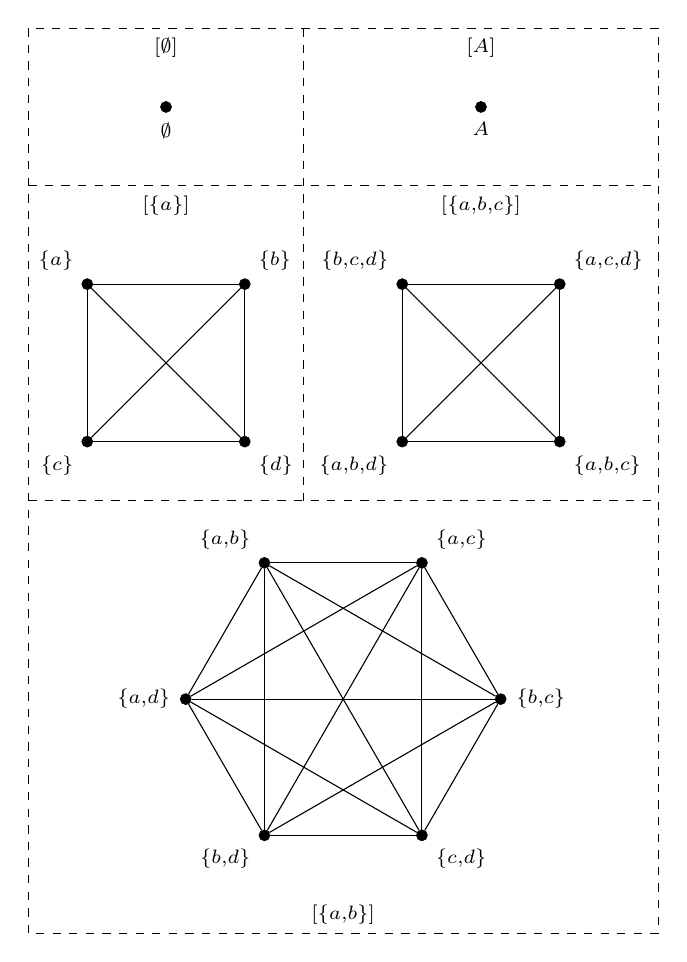
\begin{tikzpicture}[
	%scale=0.75,
	vertex/.style={ circle, draw, very thin, fill, inner sep=0pt, minimum size=4pt },
	vertexg/.style={ black!40!white, circle, draw, very thin, fill, inner sep=0pt, minimum size=4pt },
	vertexo/.style={ circle, draw, very thin, inner sep=0pt, minimum size=4pt }
]

% 0 element subset
\begin{scope}[xshift=1cm]
	\node at (0,0) (empty) [vertex,label=below:$\scriptstyle \emptyset$] {};
\end{scope}

\begin{scope}[yshift=-4.25cm]
	% 1 element subsets
	\node at (0,2) (c1a) [vertex,label=above left:{$\scriptstyle \{a\}$}] {};
	\node at (2,2) (c1b) [vertex,label=above right:{$\scriptstyle \{b\}$}] {};
	\node at (0,0) (c1c) [vertex,label=below left:{$\scriptstyle \{c\}$}] {};
	\node at (2,0) (c1d) [vertex,label=below right:{$\scriptstyle \{d\}$}] {};
	\foreach \p in {c1b,c1c,c1d} \draw (c1a) to (\p);
	\foreach \p in {c1c,c1d} \draw (c1b) to (\p);
	\draw (c1c) to (c1d);
\end{scope}

\begin{scope}[xshift=1.25cm,yshift=-9.25cm]
	% 2 element subsets
	\node at (1,3.46) (c2ab) [vertex,label=above left:{$\scriptstyle \{a,b\}$}] {};
	\node at (3,3.46) (c2ac) [vertex,label=above right:{$\scriptstyle \{a,c\}$}] {};
	\node at (0,1.73) (c2ad) [vertex,label=left:{$\scriptstyle \{a,d\}$}] {};
	\node at (4,1.73) (c2bc) [vertex,label=right:{$\scriptstyle \{b,c\}$}] {};
	\node at (1,0) (c2bd) [vertex,label=below left:{$\scriptstyle \{b,d\}$}] {};
	\node at (3,0) (c2cd) [vertex,label=below right:{$\scriptstyle \{c,d\}$}] {};
	\foreach \p in {c2ac,c2ad,c2bc,c2bd,c2cd} \draw (c2ab) to (\p);
	\foreach \p in {c2ad,c2bc,c2bd,c2cd} \draw (c2ac) to (\p);
	\foreach \p in {c2bc,c2bd,c2cd} \draw (c2ad) to (\p);
	\foreach \p in {c2bd,c2cd} \draw (c2bc) to (\p);
	\draw (c2bd) to (c2cd);
\end{scope}

\begin{scope}[xshift=4cm,yshift=-4.25cm]
	% 3 element subsets
	\node at (0,2) (c3d) [vertex,label=above left:{$\scriptstyle \{b,c,d\}$}] {};
	\node at (2,2) (c3c) [vertex,label=above right:{$\scriptstyle \{a,c,d\}$}] {};
	\node at (0,0) (c3b) [vertex,label=below left:{$\scriptstyle \{a,b,d\}$}] {};
	\node at (2,0) (c3a) [vertex,label=below right:{$\scriptstyle \{a,b,c\}$}] {};
	\foreach \p in {c3c,c3b,c3a} \draw (c3d) to (\p);
	\foreach \p in {c3b,c3a} \draw (c3c) to (\p);
	\draw (c3b) to (c3a);
\end{scope}

\begin{scope}[xshift=5cm]
	% 4 element subset
	\node at (0,0) (empty) [vertex,label=below:$\scriptstyle A$] {};
\end{scope}

%
% border
\draw[dashed] (-0.75,1) to (-0.75,-10.5)
	to node[above] {$\scriptstyle [\{a,b\}]$} (7.25,-10.5)
	to (7.25,1)
	to node[below] {$\scriptstyle [A]$} (2.75,1)
	to node[below] {$\scriptstyle [\emptyset]$} (-0.75,1);
\draw[dashed] (-0.75,-1)
	to node[below] {$\scriptstyle [\{a\}]$} (2.75,-1)
	to node[below] {$\scriptstyle [\{a,b,c\}]$} (7.25,-1);
\draw[dashed] (-0.75,-5) to (7.25,-5);
\draw[dashed] (2.75,1) to (2.75,-5);

\end{tikzpicture}
